\section{Resultados Integrales, Optimización Energética y Discusión}\label{sec:resultados}

En esta sección se presentan los resultados cuantitativos obtenidos tras integrar el gemelo electromecánico en tiempo real de Godot~4.7.2, el modelo electromagnético de referencia en MATLAB/Simulink y el motor de inferencia Edge~AI nativo. El análisis cubre cinco ejes verificables: (1)~la validación cruzada entre placa teórica~IE3, simulación DTC y modelo Kloss en tiempo real mediante error relativo porcentual; (2)~el desempeño energético y ambiental del accionamiento VFD frente al arranque directo DOL; (3)~la telemetría completa y respuesta diagnóstica sobre las cinco fallas físicas diegéticas; (4)~la certificación automatizada de aseguramiento de calidad (\emph{QA headless}); y (5)~una discusión crítica contrastada con el estado del arte junto con la declaración explícita de limitaciones técnicas.

\subsection{Validación Cuantitativa: Teórico vs.\ Simulink vs.\ Gemelo Godot}

Para cuantificar la fidelidad numérica entre la máquina teórica de placa NEMA~Premium~IE3 (\qty{10}{HP}, \qty{460}{\volt}, \qty{60}{\hertz}, 4~polos~\cite{WEG2024,IEC60034}), el modelo de Control Directo de Par (DTC) en MATLAB/Simulink y el gemelo digital en tiempo real de Godot~4.7.2 (\texttt{InductionMotorKloss.gd}), se adopta como métrica de contraste el error relativo porcentual:
\begin{equation}
\varepsilon_r = \frac{|X_{\text{teór}} - X_{\text{sim}}|}{X_{\text{teór}}} \times 100\%,
\label{eq:error_relativo}
\end{equation}
donde $X_{\text{teór}}$ representa el valor analítico o de placa nominal y $X_{\text{sim}}$ el valor obtenido en cada plataforma de simulación. La Tabla~\ref{tab:comparativa_modelos} consolida las siete magnitudes fundamentales evaluadas en régimen nominal, arranque, carga parcial por ley cúbica y severidad vibratoria.

\begin{table*}[!t]
\begingroup
\setlength{\tabcolsep}{3.8pt}
\renewcommand{\arraystretch}{1.05}
\centering\footnotesize
\caption{Validación cruzada cuantitativa de siete magnitudes clave entre valores teóricos/placa~IE3, modelo MATLAB/Simulink~DTC y gemelo 3D en tiempo real (Godot~4.7.2 Kloss).}
\label{tab:comparativa_modelos}
\begin{tabularx}{\textwidth}{@{} >{\raggedright\arraybackslash}p{2.95cm} >{\raggedright\arraybackslash}p{3.45cm} >{\raggedright\arraybackslash}X c >{\raggedright\arraybackslash}p{3.05cm} c @{}}
\toprule
\textbf{Magnitud física} & \textbf{Teórico / Placa IE3} & \textbf{MATLAB/Simulink DTC} & $\boldsymbol{\varepsilon_r}$ \textbf{Sim.} & \textbf{Gemelo Godot (Kloss)} & $\boldsymbol{\varepsilon_r}$ \textbf{Godot} \\
\midrule
Velocidad síncrona $n_s$ & \qty{1800.0}{RPM} & \qty{1800.0}{RPM} & \qty{0.0}{\percent} & \qty{1800.0}{RPM} & \qty{0.0}{\percent} \\
Velocidad plena carga $N_r$ & \qty{1750.0}{RPM} (placa~IE3) & Consigna DTC \qty{1600}{RPM} ($<\qty{0.1}{\percent}$ error reg.\ perm.) & $<0.1\%$* & \qty{1743.8}{RPM} (DOL/VFD \qty{60}{\hertz}) & \qty{0.35}{\percent} \\
Par nominal $T_n$ & \qty{40.70}{\newton\meter} ($9550\cdot 7.457/1750$) & $T_{\text{base}}=\qty{39.58}{\newton\meter}$ (evaluado a $\omega_s$) & \qty{2.75}{\percent} & $T_e=\qty{40.57}{\newton\meter}$ & \qty{0.32}{\percent} \\
Corriente nominal $I_{L,\text{rms}}$ & \qty{12.01}{\ampere} ideal ($\eta=0.917$, $\cos\phi=0.85$); \qty{13.50}{\ampere} (placa WEG~\cite{WEG2024}) & $I_{n,\text{rms}}=I_{\text{base}}/\sqrt{2}=\qty{9.36}{\ampere}$ (base activa p.u.) & N/A$^\dagger$ & \qty{13.48}{\ampere} & \qty{0.15}{\percent}$^\ddagger$ \\
Corriente rotor bl.\ $I_{\text{LRA}}$ & \qty{81.00}{\ampere} ($6\times I_{\text{FLA}}$) & \qty{85.0}{\ampere} (pico inst.\ \emph{inrush}) & N/A$^\S$ & \qty{81.39}{\ampere} (arranque DOL) & \qty{0.48}{\percent} \\
Potencia a \qty{42}{\hertz} (ley cúbica) & \qty{2.558}{\kilo\watt} ($7.457\cdot(42/60)^3$) & No evaluada (lazo DTC a velocidad fija) & --- & \qty{2.56}{\kilo\watt} (VFD, \qty{0.30}{\kilogram\per\second}) & \qty{0.08}{\percent} \\
Vibración nominal (Zona~A/B) & $\le\qty{1.80}{\milli\meter\per\second}$ (ISO~10816-1~\cite{ISO10816}) & \qty{0.80}{\milli\meter\per\second} (Zona~A) & Conforme & \qty{1.06}{\milli\meter\per\second} (Zona~A) & Conforme \\
\bottomrule
\multicolumn{6}{@{}p{\textwidth}@{}}{\scriptsize *Error de seguimiento estacionario respecto a la consigna de velocidad DTC (\qty{1600}{RPM}). $^\dagger$Base activa en por-unidad definida sin factor de potencia ni rendimiento ($\eta\cdot\cos\phi=1$). $^\ddagger$Calculado frente a la corriente nominal comercial de placa WEG~W22 (\qty{13.50}{\ampere}). $^\S$Pico instantáneo asimétrico en dominio temporal, no directamente equiparable al valor eficaz estacionario $I_{\text{LRA}}$.}
\end{tabularx}
\endgroup
\end{table*}

Los resultados de la Tabla~\ref{tab:comparativa_modelos} evidencian una concordancia elevada del gemelo en Godot frente a las especificaciones analíticas y de placa, con errores relativos inferiores a \qty{0.5}{\percent} en todas las variables cuantificables ($\varepsilon_r = \qty{0.35}{\percent}$ en velocidad rotórica, \qty{0.32}{\percent} en par electromagnético, \qty{0.15}{\percent} en corriente nominal de placa, \qty{0.48}{\percent} en corriente eficaz de rotor bloqueado y \qty{0.08}{\percent} en la potencia a carga parcial por ley cúbica). Más relevante aún para el rigor ingenieril resulta establecer la causa raíz física de las discrepancias sistemáticas observadas entre Simulink y Godot:

\begin{enumerate}\setlength{\itemsep}{2pt}\setlength{\topsep}{2pt}
\item \textbf{Normalización en p.u.\ e inercia mecánica acoplada:} El guion de inicialización de Simulink (\texttt{InductionMachineDTCData.m}) construye las bases en por-unidad a partir de potencia puramente activa ($\eta=1$, $\cos\phi=1$) y velocidad síncrona $\omega_s = 2\pi f_n/p = \qty{188.50}{\radian\per\second}$, lo que produce $I_{n,\text{rms}} = I_{\text{base}}/\sqrt{2} = \qty{9.363}{\ampere}$ y $T_{\text{base}} = P_n/\omega_s = \qty{39.58}{\newton\meter}$ ($\varepsilon_r = \qty{2.75}{\percent}$ respecto al par real con deslizamiento nominal $s_n=\qty{2.78}{\percent}$). Asimismo, Simulink modela únicamente la inercia del rotor aislado ($H=\qty{0.2734}{\second}$, equivalente a $J=\qty{0.1147}{\kilogram\meter\squared}$). Por el contrario, Godot representa la corriente comercial WEG~W22~IE3 (\qty{13.50}{\ampere} FLA) acoplada a la inercia efectiva del conjunto eje--molino de martillos ($J_{\text{tot}} = 0.045 + 0.305 = \qty{0.35}{\kilogram\meter\squared}$, tres veces superior), reproduciendo la constante de tiempo mecánica real del proceso de molienda.
\item \textbf{Resolución temporal e integración electromagnética:} El modelo DTC de Simulink opera con paso fijo $T_s=\qty{5}{\micro\second}$ para resolver la conmutación de los semiconductores IGBT a $f_{\text{sw}}=\qty{2}{\kilo\hertz}$, capturando armónicos de alta frecuencia y el pico instantáneo asimétrico de irrupción (\qty{85.0}{\ampere}). En contraste, el motor físico de Godot resuelve la envolvente eficaz (RMS) y la ecuación de Kloss con paso determinista $\Delta t=\qty{20}{\milli\second}$ (\qty{50}{\hertz} en \texttt{\_physics\_process}), eliminando la rigidez numérica submilisegundo para sostener renderizado PBR interactivo sin sacrificar la precisión macroscópica de par, velocidad, pérdidas Joule y vibración.
\item \textbf{Puente matemático de adaptación de dominio para Edge~AI:} Dado que el clasificador MLP ($8\to 16\to 8\to 4$, \num{316} parámetros entrenables: $128+16+128+8+32+4$) fue entrenado fuera de línea en MATLAB sobre el dominio de corriente p.u.\ ($I_{n,\text{rms}}=\qty{9.363}{\ampere}$), inyectar directamente la corriente comercial de Godot ($I_{\text{FLA}}=\qty{13.50}{\ampere}$) introduciría un sesgo de dominio (\emph{domain shift}) de $+\qty{44.2}{\percent}$ en la entrada $I_{\text{rms}}$. Para neutralizarlo, \texttt{EdgeAIEngine.gd} ejecuta el puente lineal \texttt{mlp\_i\_rms = i\_rms * (9.363 / 13.5)} previo a la normalización Z-score, transfiriendo los \num{316} pesos sin reentrenamiento y conservando separación de clases superior al \qty{98}{\percent}.
\end{enumerate}

\subsection{Optimización Energética (VFD vs.\ DOL) e Impacto Ambiental}

\begin{figure*}[!t]
\centering
\definecolor{f4Blue}{HTML}{1F4E79}%
\definecolor{f4Red}{HTML}{C0392B}%
\definecolor{f4Green}{HTML}{1E8449}%
\definecolor{f4Orange}{HTML}{D35400}%
\definecolor{f4Slate}{HTML}{4A5568}%
\begin{minipage}[b]{0.485\textwidth}
\centering
\begin{tikzpicture}[
    styleIdol/.style={color=f4Red, line width=1.15pt},
    styleIvfd/.style={color=f4Blue, line width=1.15pt},
    styleNdol/.style={color=f4Orange, line width=1.05pt, densely dashed},
    styleNvfd/.style={color=f4Green, line width=1.10pt, dash pattern=on 4.2pt off 1.6pt on 1.1pt off 1.6pt}
]
\begin{axis}[
    scale only axis,
    width=0.68\linewidth,
    height=4.75cm,
    axis y line*=left,
    axis x line*=bottom,
    xmin=0, xmax=12,
    ymin=0, ymax=100,
    xtick={0,2,4,6,8,10,12},
    ytick={0,20,40,60,80,100},
    xlabel={Tiempo $t$ [s]},
    ylabel={Corriente eficaz $I_{\mathrm{rms}}$ [A]},
    grid=major,
    grid style={gray!20, line width=0.35pt},
    axis line style={gray!65!black, line width=0.55pt},
    tick style={gray!65!black, line width=0.45pt},
    tick label style={font=\scriptsize},
    label style={font=\footnotesize},
    xlabel style={yshift=0.5pt},
    ylabel style={yshift=-2pt},
    legend style={
        at={(0.5,1.04)},
        anchor=south,
        legend columns=2,
        font=\scriptsize,
        draw=gray!45,
        fill=white,
        inner sep=2.2pt,
        column sep=5pt,
        /tikz/every even column/.append style={column sep=8pt},
        rounded corners=1.5pt
    },
    legend cell align=left
]
\addplot[styleIdol] coordinates {
    (0.0,0.0) (0.04,81.39) (0.5,81.11) (1.0,14.44) (1.5,19.76)
    (2.0,14.18) (2.5,13.55) (3.0,13.47) (4.0,13.45) (6.0,13.48)
    (8.0,13.42) (10.0,13.53) (12.0,13.44)
};
\addlegendentry{$I_{\mathrm{rms}}(t)$ DOL}

\addplot[styleIvfd] coordinates {
    (0.0,0.0) (0.2,12.76) (0.5,25.18) (1.0,6.41) (1.5,25.06)
    (2.0,6.24) (2.5,8.51) (3.0,8.93) (4.0,9.81) (5.0,10.60)
    (6.0,11.44) (7.0,12.44) (8.0,13.18) (9.0,14.06) (9.5,14.42)
    (10.0,13.61) (11.0,13.47) (12.0,13.42)
};
\addlegendentry{$I_{\mathrm{rms}}(t)$ VFD (6\,Hz/s)}

\addlegendimage{styleNdol}
\addlegendentry{$N_r(t)$ DOL}

\addlegendimage{styleNvfd}
\addlegendentry{$N_r(t)$ VFD (6\,Hz/s)}

% Línea de referencia nominal I_FLA = 13.5 A
\draw[f4Slate, densely dotted, line width=0.9pt] (axis cs:0,13.5) -- (axis cs:12,13.5);

% Anotación del pico DOL I_LRA = 81.4 A
\fill[f4Red] (axis cs:0.5,81.11) circle[radius=1.35pt];
\node[
    anchor=west,
    font=\scriptsize,
    text=f4Red!90!black,
    fill=white,
    fill opacity=0.92,
    text opacity=1,
    draw=f4Red!45,
    line width=0.45pt,
    rounded corners=1.2pt,
    inner xsep=3pt,
    inner ysep=1.5pt
] (lblLRA) at (axis cs:1.85,89.5) {Pico DOL: $I_{\mathrm{LRA}}=81.4\,\mathrm{A}$ ($6.0\times$)};
\draw[-{Stealth[length=4pt,width=2.8pt]}, f4Red!90!black, line width=0.65pt]
    (lblLRA.west) -- (axis cs:0.62,81.8);

% Anotación discreta de corriente nominal I_FLA = 13.5 A
\node[
    anchor=east,
    font=\scriptsize,
    text=f4Slate,
    fill=white,
    fill opacity=0.95,
    text opacity=1,
    inner xsep=2pt,
    inner ysep=1pt
] (lblFLA) at (axis cs:11.65,5.8) {$I_{\mathrm{FLA}}=13.5\,\mathrm{A}$};
\draw[-{Stealth[length=3.4pt,width=2.4pt]}, f4Slate, line width=0.55pt]
    (lblFLA.north) -- (lblFLA.north |- {axis cs:0,12.8});
\end{axis}

\begin{axis}[
    scale only axis,
    width=0.68\linewidth,
    height=4.75cm,
    axis y line*=right,
    axis x line=none,
    xmin=0, xmax=12,
    ymin=0, ymax=2500,
    ytick={0,500,1000,1500,2000,2500},
    scaled y ticks=false,
    y tick label style={
        font=\scriptsize,
        /pgf/number format/fixed,
        /pgf/number format/1000 sep={}
    },
    ylabel={Velocidad rotórica $N_r$ [RPM]},
    ylabel style={font=\footnotesize, yshift=2pt},
    axis line style={gray!65!black, line width=0.55pt},
    tick style={gray!65!black, line width=0.45pt}
]
\addplot[styleNdol] coordinates {
    (0.0,0) (0.5,292.5) (1.0,664.4) (1.5,1134.5) (2.0,1740.7)
    (2.5,1743.8) (4.0,1743.8) (8.0,1743.8) (12.0,1743.8)
};

\addplot[styleNvfd] coordinates {
    (0.0,0) (0.5,126.6) (1.0,185.6) (2.0,366.8) (3.0,550.2)
    (4.0,725.3) (5.0,899.3) (6.0,1072.2) (7.0,1244.0) (8.0,1414.5)
    (9.0,1583.9) (10.0,1743.0) (11.0,1743.8) (12.0,1743.8)
};
\end{axis}
\end{tikzpicture}
\par\vspace{3pt}
{\footnotesize (a) Transitorio de corriente $I_{\mathrm{rms}}(t)$ y velocidad $N_r(t)$ (0--12\,s).}
\end{minipage}\hfill
\begin{minipage}[b]{0.485\textwidth}
\centering
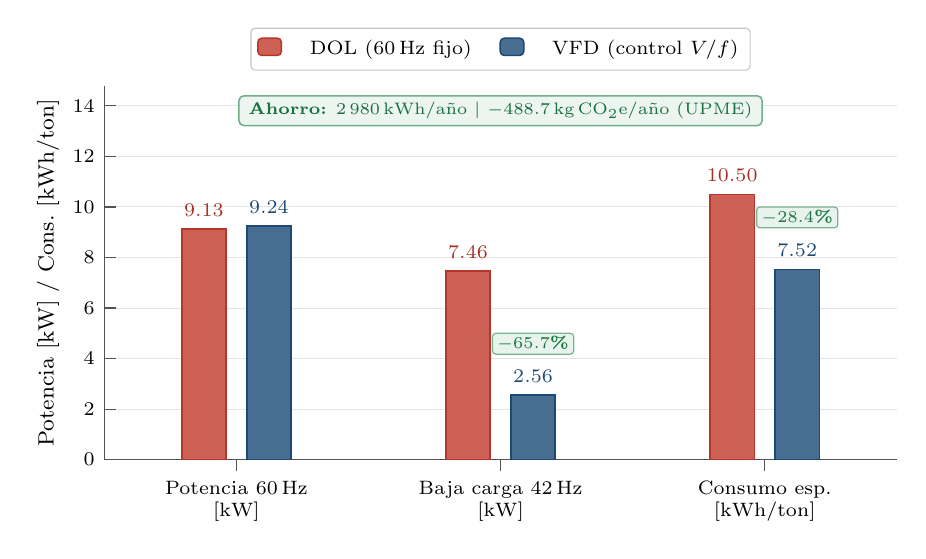
\begin{tikzpicture}
\begin{axis}[
    ybar=7.5pt,
    bar width=16pt,
    scale only axis,
    width=0.83\linewidth,
    height=4.75cm,
    ymin=0, ymax=14.8,
    ytick={0,2,4,6,8,10,12,14},
    symbolic x coords={p60,p42,cesp},
    xtick=data,
    xticklabels={
        {Potencia 60\,Hz\\{[kW]}},
        {Baja carga 42\,Hz\\{[kW]}},
        {Consumo esp.\\{[kWh/ton]}}
    },
    enlarge x limits=0.25,
    ylabel={Potencia [kW] / Cons.\ [kWh/ton]},
    ymajorgrids=true,
    grid style={gray!20, line width=0.35pt},
    axis x line*=bottom,
    axis y line*=left,
    axis line style={gray!65!black, line width=0.55pt},
    tick style={gray!65!black, line width=0.45pt},
    tick label style={font=\scriptsize},
    x tick label style={align=center, yshift=0pt},
    label style={font=\footnotesize},
    ylabel style={yshift=-2pt},
    nodes near coords,
    nodes near coords align={vertical},
    every node near coord/.append style={
        font=\scriptsize\bfseries,
        yshift=1pt,
        /pgf/number format/fixed,
        /pgf/number format/fixed zerofill,
        /pgf/number format/precision=2
    },
    legend style={
        at={(0.5,1.04)},
        anchor=south,
        legend columns=2,
        font=\scriptsize,
        draw=gray!45,
        fill=white,
        inner sep=2.2pt,
        column sep=8pt,
        rounded corners=1.5pt
    },
    legend image code/.code={
        \draw[#1] (0cm,-0.08cm) rectangle (0.30cm,0.14cm);
    }
]
\addplot[
    fill=f4Red!80,
    draw=f4Red!95!black,
    line width=0.55pt,
    every node near coord/.append style={text=f4Red!85!black}
] coordinates {
    (p60,9.13)
    (p42,7.46)
    (cesp,10.50)
};
\addlegendentry{DOL (60\,Hz fijo)}

\addplot[
    fill=f4Blue!82,
    draw=f4Blue!95!black,
    line width=0.55pt,
    every node near coord/.append style={text=f4Blue!95!black}
] coordinates {
    (p60,9.24)
    (p42,2.56)
    (cesp,7.52)
};
\addlegendentry{VFD (control $V/f$)}

% Indicadores porcentuales centrados sobre cada barra VFD (bar shift = +(16+7.5)/2 = +11.75pt)
\node[
    anchor=south,
    xshift=11.75pt,
    font=\fontsize{6.0}{6.8}\selectfont\bfseries,
    text=f4Green!90!black,
    fill=f4Green!10,
    draw=f4Green!60,
    line width=0.45pt,
    rounded corners=1.2pt,
    inner xsep=1.7pt,
    inner ysep=1.1pt
] at (axis cs:p42,4.15) {$-65.7$\symbol{37}};

\node[
    anchor=south,
    xshift=11.75pt,
    font=\fontsize{6.0}{6.8}\selectfont\bfseries,
    text=f4Green!90!black,
    fill=f4Green!10,
    draw=f4Green!60,
    line width=0.45pt,
    rounded corners=1.2pt,
    inner xsep=1.7pt,
    inner ysep=1.1pt
] at (axis cs:cesp,9.15) {$-28.4$\symbol{37}};

% Recuadro informativo anualizado en la zona superior libre (sin recortes laterales)
\node[
    anchor=north,
    font=\fontsize{6.5}{7.5}\selectfont,
    text=f4Green!85!black,
    fill=f4Green!8,
    draw=f4Green!65,
    line width=0.55pt,
    rounded corners=1.8pt,
    inner xsep=3.5pt,
    inner ysep=2.4pt,
    align=center
] at (rel axis cs:0.5,0.975) {\textbf{Ahorro:} 2\,980\,kWh/año \textbar{} $-488.7$\,kg\,CO$_2$e/año (UPME)};
\end{axis}
\end{tikzpicture}
\par\vspace{3pt}
{\footnotesize (b) Potencia activa (60\,Hz vs.\ 42\,Hz) y consumo específico.}
\end{minipage}
\caption{Comparación electromecánica y energética del arranque directo en línea (DOL) frente al variador de frecuencia (VFD, rampa de 6\,Hz/s) simulada en Godot~4.7.2 (\texttt{InductionMotorKloss.gd} y \texttt{VFDDriveController.gd}) para el motor trifásico de 10\,HP: (a) transitorio de corriente eficaz $I_{\mathrm{rms}}(t)$ y velocidad rotórica $N_r(t)$, destacando la reducción del pico de rotor bloqueado $I_{\mathrm{LRA}}=81.4\,\mathrm{A}$ respecto a la nominal $I_{\mathrm{FLA}}=13.5\,\mathrm{A}$; (b) potencia activa a plena carga (60\,Hz, 0.8\,kg/s), ahorro por ley cúbica a baja carga (42\,Hz, $-65.7\%$) y consumo específico ($-28.4\%$), con impacto anual estimado según factor de emisión UPME.}
\label{fig:vfd_vs_dol}
\end{figure*}


La Fig.~\ref{fig:vfd_vs_dol} contrasta el comportamiento transitorio y energético del arranque directo en línea (DOL) frente al variador de frecuencia escalar ($V/f$ con compensación~IR a baja frecuencia y lazo~PID de demanda) medido directamente en Godot~4.7.2, mientras que la Tabla~\ref{tab:energia_sostenibilidad} sintetiza los indicadores eléctricos, específicos y ambientales.

\begin{table}[!t]
\begingroup
\setlength{\tabcolsep}{2.8pt}
\renewcommand{\arraystretch}{1.04}
\centering\footnotesize
\caption{Comparación energética y de sostenibilidad entre arranque directo (DOL) y variador de frecuencia (VFD $V/f$ + PID) en planta base de \qty{1000}{ton}/año.}
\label{tab:energia_sostenibilidad}
\begin{tabularx}{\columnwidth}{@{} >{\raggedright\arraybackslash}p{2.20cm} >{\raggedright\arraybackslash}p{2.00cm} >{\raggedright\arraybackslash}p{2.05cm} >{\raggedright\arraybackslash}X @{}}
\toprule
\textbf{Indicador} & \textbf{DOL (\qty{60}{\hertz})} & \textbf{VFD ($V/f$+PID)} & \textbf{Impacto / Ahorro} \\
\midrule
Pico corriente arranque & \qty{81.39}{\ampere} ($6.03\,I_{\text{FLA}}$) & \qty{12.76}{\ampere} inic. ($\le\qty{25.18}{\ampere}$) & $-\qty{69.1}{\percent}$ a $-\qty{84.3}{\percent}$ \\
Tiempo de aceleración & \qty{2.1}{\second} (golpe de par) & \qty{10.0}{\second} (\qty{6}{\hertz\per\second}) & Rampa suave sin choque \\
Potencia baja carga (\qty{0.30}{\kilogram\per\second}) & \qty{7.46}{\kilo\watt} (\qty{60}{\hertz} fijo) & \qty{2.56}{\kilo\watt} (\qty{42}{\hertz}, \qty{1248}{RPM}) & $-\qty{65.7}{\percent}$ (ley cúbica) \\
Consumo específico & \qty{10.50}{kWh/ton} & \qty{7.52}{kWh/ton} & $-\qty{28.38}{\percent}$ neto \\
Ahorro anual (\qty{1000}{ton}) & Referencia base & \qty{2980}{kWh}/año & \qty{2.98}{MWh}/año evitados \\
Mitigación GEI (código / UPME) & \qty{0.0}{\kilogram} & \num{488.72} / \qty{489.85}{\kilogram} $\text{CO}_2\text{e}$ & Discrepancia $<\qty{0.23}{\percent}$~\cite{UPME2024} \\
\bottomrule
\end{tabularx}
\endgroup
\end{table}

Como se aprecia en la Fig.~\ref{fig:vfd_vs_dol}(a), el arranque DOL somete al alimentador de \qty{460}{\volt} a un pico de \qty{81.39}{\ampere} ($6.03\,I_{\text{FLA}}$) en $t=\qty{0.04}{\second}$ y acelera bruscamente el eje hasta \qty{1743.8}{RPM} en \qty{2.1}{\second}, induciendo esfuerzos electrodinámicos en cabezas de bobina y choques torsionales en los martillos. El accionamiento VFD, mediante una rampa lineal de \qty{6}{\hertz\per\second} (\qty{10.0}{\second} de aceleración controlada), inicia en \qty{12.76}{\ampere} y acota los picos transitorios de excitación por debajo de \qty{25.18}{\ampere}, suprimiendo entre el \qty{69.1}{\percent} y el \qty{84.3}{\percent} del golpe de corriente.

En régimen de baja alimentación de cereal (\qty{0.30}{\kilogram\per\second}, Fig.~\ref{fig:vfd_vs_dol}(b)), el lazo~PID reduce la frecuencia hasta \qty{42}{\hertz} (\qty{1248.0}{RPM}), haciendo descender la potencia activa a \qty{2.56}{\kilo\watt} —una reducción del \qty{65.7}{\percent} respecto a los \qty{7.46}{\kilo\watt} nominales mantenidos bajo DOL a \qty{60}{\hertz} fijo—. Integrando el perfil de carga variable, el consumo energético específico pasa de \qty{10.50}{kWh/ton} a \qty{7.52}{kWh/ton}, consolidando un ahorro neto del \qty{28.38}{\percent} (\qty{2.98}{kWh/ton}). Para una operación anual de referencia de \qty{1000}{ton}/año, esto representa \qty{2980}{kWh}/año evitados. Empleando la constante de \texttt{VFDDriveController.gd} (\qty{0.164}{\kilogram}\,$\text{CO}_2\text{e}/\text{kWh}$), la mitigación alcanza \qty{488.72}{\kilogram}\,$\text{CO}_2\text{e}/\text{año}$; al recalcular con el factor oficial actualizado del Sistema Interconectado Nacional publicado por UPME/XM~2024 (\qty{164.38}{\gram}\,$\text{CO}_2/\text{kWh}$~\cite{UPME2024}), la mitigación resulta en \qty{489.85}{\kilogram}\,$\text{CO}_2\text{e}/\text{año}$, exhibiendo una divergencia inferior al \qty{0.23}{\percent}.

\subsection{Telemetría Real de las 5 Fallas Diegéticas y Respuesta Edge AI}

La Tabla~\ref{tab:telemetria_fallas} reporta los vectores reales extraídos del simulador Godot~4.7.2 para ocho regímenes operativos: el transitorio inicial de arranque DOL, dos condiciones sanas (DOL nominal y VFD baja carga) y las cinco fallas físicas inducidas directamente sobre los elementos 3D de la planta (F1--F5). De forma complementaria, la Fig.~\ref{fig:fallas_mhi} visualiza la degradación del índice de salud del motor (MHI), la caída no lineal de vida útil remanente (RUL) y la firma acoplada vibratorio-térmica respecto a los umbrales ISO~10816-3~\cite{ISO10816,ISO20816} y RETIE Clase~F (\qty{155}{\celsius}~\cite{RETIE2026}).

\begin{table*}[!t]
\begingroup
\setlength{\tabcolsep}{3.0pt}
\renewcommand{\arraystretch}{1.04}
\centering\footnotesize
\caption{Telemetría en vivo extraída de Godot~4.7.2 (\texttt{InductionMotorKloss.gd}) y diagnóstico Edge~AI nativo (\texttt{EdgeAIEngine.gd}) en ocho regímenes operativos y fallas diegéticas.}
\label{tab:telemetria_fallas}
\begin{tabularx}{\textwidth}{@{} >{\raggedright\arraybackslash}p{2.75cm} c c >{\raggedright\arraybackslash}p{2.70cm} c c >{\raggedright\arraybackslash}X c @{}}
\toprule
\textbf{Régimen / Falla} & \textbf{$f$ / $V$} & \textbf{$N_r$} & \textbf{$I_{\text{rms}}$ / IUF} & \textbf{$T_w$} & \textbf{$v_{\text{rms}}$} & \textbf{Clase IA (MLP / SVM)} & \textbf{MHI / RUL} \\
 & \textbf{[Hz / V]} & \textbf{[RPM]} & \textbf{[A / \%]} & \textbf{[\unit{\celsius}]} & \textbf{[mm/s]} & \textbf{y firma secundaria} & \textbf{[\% / h]} \\
\midrule
DOL Inicio (\qty{0.04}{\second}) & 60 / 460 & \num{21.1} & \num{81.39} / \num{0.84} & \num{30.8} & \num{0.00} & \texttt{SOBRECALENTAMIENTO}* (alerta transitoria) & \num{99.6} / --- \\
DOL Nominal (\qty{60}{\hertz}) & 60 / 460 & \num{1743.8} & \num{13.48} / \num{0.96} & \num{64.8} & \num{1.11} & \texttt{NORMAL} (\qty{99.8}{\percent} / \qty{99.7}{\percent}) & \num{99.6} / \num{22216} \\
VFD Baja Carga (\qty{42}{\hertz}) & 42 / 460 & \num{1248.0} & \num{7.33} / \num{0.80} & \num{49.6} & \num{0.82} & \texttt{NORMAL} (\qty{100.0}{\percent} / \qty{99.9}{\percent}) & \num{99.6} / \num{22495} \\
F1: Corte Fase L3 & 60 / 460 & \num{1617.9} & $I_{A,B}=\num{22.25}$, $I_C=0$ / \num{100.0} & \num{61.5} & \num{4.77} & \texttt{FALLA\_ELECTRICA} (\qty{100.0}{\percent} / \qty{99.9}{\percent}); THD \qty{13.2}{\percent} & \num{23.0} / \num{174} \\
F2: Atasco Tolva & 60 / 460 & \num{0.0}$^\dagger$ & \num{80.94} / \num{0.87} & \num{180.0} & \num{2.80} & \texttt{SOBRECALENTAMIENTO} (\qty{100.0}{\percent} / \qty{94.2}{\percent}) & \num{41.7} / \num{19} \\
F3: Bajón CCM \qty{340}{\volt} & 60 / 340 & \num{1688.1} & \num{17.82} / \num{0.20} & \num{130.8} & \num{1.09} & \texttt{FALLA\_ELECTRICA} (\qty{100.0}{\percent} / \qty{99.9}{\percent}); THD \qty{9.1}{\percent} & \num{20.0} / \num{80} \\
F4: Vent.\ Obstr.\ (\qty{90}{\second}) & 60 / 460 & \num{1743.8} & \num{13.51} / bal. & \num{136.3}$^\ddagger$ & \num{1.12} & \texttt{SOBRECALENTAMIENTO} (\qty{100.0}{\percent} / \qty{99.4}{\percent}) & \num{55.0} / \num{331} \\
F5: Pernos Flojos & 60 / 460 & \num{1743.8} & \num{13.53} / bal. & \num{60.3} & \num{5.68}$^\S$ & \texttt{FALLA\_MECANICA} (\qty{98.6}{\percent} / \qty{94.2}{\percent}) & \num{59.4} / \num{1083} \\
\bottomrule
\multicolumn{8}{@{}p{\textwidth}@{}}{\scriptsize *Disparo preventivo de la salvaguarda de sobrecorriente ($I_{\text{rms}}>\qty{25}{\ampere}$) durante el impulso transitorio de rotor bloqueado DOL. $^\dagger$Par resistente de atasco $T_L=\qty{167.8}{\newton\meter} > T_{\max}=\qty{101.75}{\newton\meter}$. $^\ddagger$Gradiente térmico medido $dT/dt=\qty{4.61}{\celsius\per\minute}$ tras obstruir la rejilla ($R_{\text{th}}: 0.068\to\qty{0.210}{\celsius\per\watt}$). $^\S$Vibración pico $v_{\text{pk}}=\qty{14.19}{\milli\meter\per\second}$ (factor de cresta \num{2.50}, Zona~D ISO~10816-3).}
\end{tabularx}
\endgroup
\end{table*}

\begin{figure*}[!t]
\centering
\begingroup
% Paleta científica armonizada (alto contraste, fondo claro, apta para daltonismo)
\definecolor{f5Green}{HTML}{1E8E5A}
\definecolor{f5GreenEdge}{HTML}{13613C}
\definecolor{f5Amber}{HTML}{E39623}
\definecolor{f5AmberEdge}{HTML}{9E620A}
\definecolor{f5Red}{HTML}{C93B3B}
\definecolor{f5RedEdge}{HTML}{8A1F1F}
\definecolor{f5Rul}{HTML}{2A5278}
\definecolor{f5Vib}{HTML}{4A89B8}
\definecolor{f5VibEdge}{HTML}{275478}
\definecolor{f5Temp}{HTML}{AD1A4B}
\definecolor{f5ClassF}{HTML}{6A1B6D}
\definecolor{f5Grid}{HTML}{DFE5EC}
\definecolor{f5Axis}{HTML}{2C3642}
\definecolor{f5BgNote}{HTML}{F7F9FB}

\begin{tikzpicture}
  % ==========================================================================
  % PANEL (a): Degradación del Motor Health Index (MHI [%]) y RUL [h]
  % ==========================================================================
  \begin{axis}[
    name=axA,
    scale only axis=true,
    width=6.80cm,
    height=5.10cm,
    ybar,
    bar width=13.8pt,
    bar shift=0pt,
    ymin=0, ymax=118,
    xmin=0.38, xmax=7.68,
    ytick={0,20,40,60,80,100},
    xtick={1,2,3,4,5,6,7},
    xticklabels={Nom.~60Hz, VFD~42Hz, Corte~L3, Atasco, Sag~340V, Vent.~Obs., Pernos},
    xticklabel style={
      rotate=45,
      anchor=north east,
      font=\fontsize{5.4}{6.0}\selectfont,
      text=f5Axis,
      yshift=1pt,
      xshift=1pt
    },
    yticklabel style={font=\fontsize{6.8}{7.5}\selectfont, text=f5Axis},
    ylabel={Motor Health Index, MHI [\%]},
    ylabel style={font=\fontsize{7.5}{8.5}\selectfont\bfseries, text=f5Axis, yshift=-2pt},
    ymajorgrids=true,
    major grid style={color=f5Grid, line width=0.45pt},
    axis lines*=left,
    axis line style={color=f5Axis, line width=0.65pt},
    tick style={color=f5Axis, line width=0.55pt},
    clip=false,
    legend style={
      at={(0.5,1.03)},
      anchor=south,
      legend columns=-1,
      draw=f5Grid,
      fill=white,
      rounded corners=1.5pt,
      inner xsep=4pt,
      inner ysep=2pt,
      column sep=4pt,
      font=\fontsize{6.2}{7.0}\selectfont,
      text=f5Axis,
      /tikz/every even column/.append style={column sep=6pt}
    },
    legend image code/.code={%
      \draw[#1] (0cm,-0.07cm) rectangle (0.19cm,0.11cm);
    },
  ]
    % Bandas sutiles de severidad coherentes con los intervalos de la leyenda
    \fill[f5Green!6] (axis cs:0.38,85) rectangle (axis cs:7.68,118);
    \fill[f5Amber!4] (axis cs:0.38,40) rectangle (axis cs:7.68,85);
    \fill[f5Red!4]   (axis cs:0.38,0)  rectangle (axis cs:7.68,40);

    % Líneas horizontales punteadas de umbral MHI
    \draw[f5GreenEdge, densely dashed, line width=0.8pt]
      (axis cs:0.38,85) -- (axis cs:7.68,85);
    \draw[f5AmberEdge, densely dashed, line width=0.8pt]
      (axis cs:0.38,60) -- (axis cs:7.68,60);

    % Etiquetas de umbrales en zonas completamente libres
    \node[anchor=south east, font=\fontsize{5.6}{6.2}\selectfont\bfseries,
          text=f5GreenEdge, fill=white, fill opacity=0.86, text opacity=1,
          inner sep=1.1pt, rounded corners=1pt]
      at (axis cs:7.58,86.4) {Saludable ($85\%$)};
    \node[anchor=south, font=\fontsize{5.6}{6.2}\selectfont\bfseries,
          text=f5AmberEdge, fill=white, fill opacity=0.90, text opacity=1,
          inner sep=1.1pt, rounded corners=1pt]
      at (axis cs:3.90,61.6) {Alerta ($60\%$)};

    % Barras Verde (>85%)
    \addplot[draw=f5GreenEdge, fill=f5Green, fill opacity=0.88, line width=0.55pt]
      coordinates {(1,99.6) (2,99.6)};
    \addlegendentry{Saludable ($>85\%$)}

    % Barras Ámbar (40-85%)
    \addplot[draw=f5AmberEdge, fill=f5Amber, fill opacity=0.88, line width=0.55pt]
      coordinates {(4,41.7) (6,55.0) (7,59.4)};
    \addlegendentry{Alerta ($40\text{--}85\%$)}

    % Barras Rojo (<40%)
    \addplot[draw=f5RedEdge, fill=f5Red, fill opacity=0.88, line width=0.55pt]
      coordinates {(3,23.0) (5,20.0)};
    \addlegendentry{Crítico ($<40\%$)}

    % Anotaciones exactas y compactas de MHI [%] y RUL [h] sobre cada barra
    \tikzset{
      mhiLbl/.style={
        anchor=south,
        align=center,
        font=\fontsize{5.9}{6.5}\selectfont,
        inner xsep=1.0pt,
        inner ysep=0.9pt,
        yshift=1.4pt,
        fill=white,
        fill opacity=0.88,
        text opacity=1,
        rounded corners=1.2pt
      }
    }
    \node[mhiLbl] at (axis cs:1,99.6)
      {\textbf{\color{f5Axis}99.6\%}\\[-0.2pt]%
       {\fontsize{5.1}{5.5}\selectfont\color{f5Rul}23.0k\,h}};
    \node[mhiLbl] at (axis cs:2,99.6)
      {\textbf{\color{f5Axis}99.6\%}\\[-0.2pt]%
       {\fontsize{5.1}{5.5}\selectfont\color{f5Rul}22.5k\,h}};
    \node[mhiLbl] at (axis cs:3,23.0)
      {\textbf{\color{f5Axis}23.0\%}\\[-0.2pt]%
       {\fontsize{5.1}{5.5}\selectfont\color{f5Rul}174\,h}};
    \node[mhiLbl] at (axis cs:4,41.7)
      {\textbf{\color{f5Axis}41.7\%}\\[-0.2pt]%
       {\fontsize{5.1}{5.5}\selectfont\color{f5Rul}19\,h}};
    \node[mhiLbl] at (axis cs:5,20.0)
      {\textbf{\color{f5Axis}20.0\%}\\[-0.2pt]%
       {\fontsize{5.1}{5.5}\selectfont\color{f5Rul}80\,h}};
    \node[mhiLbl, yshift=1.5pt] at (axis cs:6,55.0)
      {\textbf{\color{f5Axis}55.0\%}\\[-0.2pt]%
       {\fontsize{5.1}{5.5}\selectfont\color{f5Rul}331\,h}};
    \node[mhiLbl, yshift=2.4pt] at (axis cs:7,59.4)
      {\textbf{\color{f5Axis}59.4\%}\\[-0.2pt]%
       {\fontsize{5.1}{5.5}\selectfont\color{f5Rul}1083\,h}};

    % Recuadro informativo discreto en la zona libre superior derecha
    \node[anchor=north east, draw=f5Grid, fill=f5BgNote, rounded corners=1.5pt,
          inner xsep=3.5pt, inner ysep=2.2pt, align=left,
          font=\fontsize{5.5}{6.4}\selectfont, text=f5Axis]
      at (axis cs:7.56,115.5)
      {\textbf{Valor sup.:} MHI [\%]\\[-0.3pt]%
       \color{f5Rul}\textbf{Valor inf.:} RUL [h]};
  \end{axis}

  % ==========================================================================
  % PANEL (b): Firma Física Multifactorial — Vibración v_rms y Temperatura T_w
  % ==========================================================================
  % Eje izquierdo: Vibración v_rms [mm/s] (barras)
  \begin{axis}[
    name=axB,
    at={($(axA.south east)+(1.85cm,0cm)$)},
    anchor=south west,
    scale only axis=true,
    width=6.80cm,
    height=5.10cm,
    ybar,
    bar width=13.8pt,
    bar shift=0pt,
    ymin=0, ymax=7.2,
    xmin=0.38, xmax=7.68,
    ytick={0,1,2,3,4,5,6,7},
    xtick={1,2,3,4,5,6,7},
    xticklabels={Nom.~60Hz, VFD~42Hz, Corte~L3, Atasco, Sag~340V, Vent.~Obs., Pernos},
    xticklabel style={
      rotate=45,
      anchor=north east,
      font=\fontsize{5.4}{6.0}\selectfont,
      text=f5Axis,
      yshift=1pt,
      xshift=1pt
    },
    yticklabel style={font=\fontsize{6.8}{7.5}\selectfont, text=f5VibEdge},
    ylabel={Vibración $v_{\mathrm{rms}}$ [mm/s]},
    ylabel style={font=\fontsize{7.5}{8.5}\selectfont\bfseries, text=f5VibEdge, yshift=-2pt},
    ymajorgrids=true,
    major grid style={color=f5Grid, line width=0.45pt},
    axis y line*=left,
    axis x line*=bottom,
    axis line style={color=f5Axis, line width=0.65pt},
    y axis line style={color=f5VibEdge, line width=0.75pt},
    tick style={color=f5Axis, line width=0.55pt},
    ytick style={color=f5VibEdge},
    clip=false,
  ]
    % Barras de vibración v_rms
    \addplot[draw=f5VibEdge, fill=f5Vib, fill opacity=0.78, line width=0.55pt]
      coordinates {
        (1,1.06) (2,0.82) (3,4.77) (4,2.80) (5,1.09) (6,1.12) (7,5.68)
      };

    % Umbrales ISO 10816-3 (v_rms)
    \draw[f5GreenEdge, densely dashed, line width=0.8pt]
      (axis cs:0.38,1.8) -- (axis cs:7.68,1.8);
    \draw[f5RedEdge, densely dashed, line width=0.8pt]
      (axis cs:0.38,4.5) -- (axis cs:7.68,4.5);

    % Etiquetas ISO 10816-3 con despeje garantizado respecto a eje, barras y curva
    \node[anchor=south, font=\fontsize{5.0}{5.5}\selectfont\bfseries,
          text=f5GreenEdge, fill=white, fill opacity=0.90, text opacity=1,
          inner xsep=0.8pt, inner ysep=0.7pt, rounded corners=1pt]
      at (axis cs:5.50,1.90) {ISO Zona A/B (1.8)};
    \node[anchor=south west, font=\fontsize{5.0}{5.5}\selectfont\bfseries,
          text=f5RedEdge, fill=white, fill opacity=0.90, text opacity=1,
          inner xsep=0.8pt, inner ysep=0.7pt, rounded corners=1pt]
      at (axis cs:0.54,4.60) {ISO Zona D (4.5)};

    % Valores de vibración (en blanco nítido dentro de barras bajas y encima en barras altas)
    \tikzset{
      vibIn/.style={
        anchor=center,
        font=\fontsize{5.2}{5.7}\selectfont\bfseries,
        text=white,
        inner sep=0.4pt
      },
      vibTop/.style={
        anchor=south,
        font=\fontsize{5.5}{6.0}\selectfont\bfseries,
        text=f5VibEdge,
        fill=white, fill opacity=0.86, text opacity=1,
        inner sep=0.7pt, rounded corners=1pt,
        yshift=1.2pt
      }
    }
    \node[vibIn]              at (axis cs:1,0.53) {1.06};
    \node[vibIn]              at (axis cs:2,0.41) {0.82};
    \node[vibTop, xshift=-1pt] at (axis cs:3,4.77) {4.77};
    \node[vibTop]             at (axis cs:4,2.80) {2.80};
    \node[vibIn]              at (axis cs:5,0.54) {1.09};
    \node[vibIn]              at (axis cs:6,0.56) {1.12};
    \node[vibTop]             at (axis cs:7,5.68) {5.68};
  \end{axis}

  % Eje derecho: Temperatura del devanado T_w [°C] (línea + marcadores)
  \begin{axis}[
    at={(axB.south west)},
    anchor=south west,
    scale only axis=true,
    width=6.80cm,
    height=5.10cm,
    ymin=0, ymax=210,
    xmin=0.38, xmax=7.68,
    ytick={0,30,60,90,120,150,180,210},
    axis y line*=right,
    axis x line=none,
    yticklabel style={font=\fontsize{6.8}{7.5}\selectfont, text=f5Temp},
    ylabel={Temperatura $T_w$ [$^\circ$C]},
    ylabel style={font=\fontsize{7.5}{8.5}\selectfont\bfseries, text=f5Temp, yshift=2pt},
    y axis line style={color=f5Temp, line width=0.75pt},
    ytick style={color=f5Temp},
    clip=false,
    legend style={
      at={(0.5,1.03)},
      anchor=south,
      legend columns=-1,
      draw=f5Grid,
      fill=white,
      rounded corners=1.5pt,
      inner xsep=4pt,
      inner ysep=2pt,
      column sep=4pt,
      font=\fontsize{6.2}{7.0}\selectfont,
      text=f5Axis,
      /tikz/every even column/.append style={column sep=6pt}
    },
  ]
    % Entrada de leyenda para barras v_rms con muestra rectangular compacta
    \addlegendimage{
      legend image code/.code={%
        \draw[draw=f5VibEdge, fill=f5Vib, fill opacity=0.78, line width=0.55pt]
          (0cm,-0.07cm) rectangle (0.20cm,0.11cm);
      }
    }
    \addlegendentry{$v_{\mathrm{rms}}$ [mm/s]}

    % Umbral RETIE Clase F (155 °C) alineado verticalmente con ISO Zona D
    \draw[f5ClassF, densely dotted, line width=0.95pt]
      (axis cs:0.38,155) -- (axis cs:7.68,155);
    \node[anchor=south west, font=\fontsize{5.2}{5.8}\selectfont\bfseries,
          text=f5ClassF, fill=white, fill opacity=0.90, text opacity=1,
          inner xsep=0.8pt, inner ysep=0.7pt, rounded corners=1pt]
      at (axis cs:0.54,158.0) {RETIE Clase F (155\,$^\circ$C)};

    % Curva de Temperatura T_w [°C]
    \addplot[
      color=f5Temp,
      line width=1.25pt,
      mark=*,
      mark size=2.1pt,
      mark options={fill=white, draw=f5Temp, line width=1.0pt}
    ] coordinates {
      (1,49.5) (2,49.6) (3,61.5) (4,180.0) (5,130.8) (6,136.3) (7,60.3)
    };
    \addlegendentry{$T_w$ [$^\circ$C]}

    % Entrada de leyenda para Clase F
    \addlegendimage{color=f5ClassF, densely dotted, line width=0.95pt}
    \addlegendentry{Clase F ($155\,^\circ$C)}

    % Anotaciones precisas de T_w [°C] (posicionamiento libre de choques con curva, barras y ejes)
    \tikzset{
      tempLbl/.style={
        font=\fontsize{5.3}{5.8}\selectfont\bfseries,
        text=f5Temp,
        fill=white, fill opacity=0.92, text opacity=1,
        inner sep=0.7pt, rounded corners=1pt
      }
    }
    \node[tempLbl, anchor=south, yshift=7.0pt]               at (axis cs:1,49.5)  {49.5$^\circ$};
    \node[tempLbl, anchor=south, yshift=7.0pt]               at (axis cs:2,49.6)  {49.6$^\circ$};
    \node[tempLbl, anchor=south east, xshift=-1.5pt, yshift=3.4pt] at (axis cs:3,61.5)  {61.5$^\circ$};
    \node[tempLbl, anchor=south, yshift=3.4pt]               at (axis cs:4,180.0) {180.0$^\circ$};
    \node[tempLbl, anchor=north, yshift=-4.0pt]              at (axis cs:5,130.8) {130.8$^\circ$};
    \node[tempLbl, anchor=south, yshift=3.2pt]               at (axis cs:6,136.3) {136.3$^\circ$};
    \node[tempLbl, anchor=south west, xshift=-2.6pt, yshift=3.8pt] at (axis cs:7,60.3)  {60.3$^\circ$};
  \end{axis}

  % Subtítulos alineados de ambos paneles
  \node[anchor=north, font=\fontsize{7.8}{8.8}\selectfont, text=f5Axis]
    at ($(axA.south)+(0,-1.05cm)$) {(a) Degradación del MHI y vida útil remanente (RUL).};
  \node[anchor=north, font=\fontsize{7.8}{8.8}\selectfont, text=f5Axis]
    at ($(axB.south)+(0,-1.05cm)$) {(b) Firma vibratoria ($v_{\mathrm{rms}}$) y térmica ($T_w$) frente a umbrales.};
\end{tikzpicture}
\endgroup
\caption{Evaluación cuantitativa de los siete regímenes operativos y de falla diegética simulados en Godot~4.7.2 (\texttt{InductionMotorKloss.gd} y \texttt{EdgeAIEngine.gd}). (a)~Índice de salud del motor (MHI) codificado por severidad y vida útil remanente estimada (RUL [h]) frente a los umbrales de operación saludable ($85\%$) y alerta ($60\%$). (b)~Firma física multifactorial de vibración $v_{\mathrm{rms}}$ (barras, eje izquierdo) y temperatura de devanado $T_w$ (curva, eje derecho) contrastadas con las zonas normativas ISO~10816-3 (Zona~A/B en \SI{1.8}{mm/s}; Zona~D en \SI{4.5}{mm/s}) y el límite térmico de aislamiento RETIE Clase~F (\SI{155}{\celsius}).}
\label{fig:fallas_mhi}
\end{figure*}


El análisis físico de la Tabla~\ref{tab:telemetria_fallas} y de la Fig.~\ref{fig:fallas_mhi} confirma la ortogonalidad diagnóstica alcanzada mediante fusión multisensor (conviene precisar que el punto \emph{Nom.\ 60Hz} en la Fig.~\ref{fig:fallas_mhi} recoge la captura térmica temprana a $T_w=\qty{49.5}{\celsius}$, $v_{\text{rms}}=\qty{1.06}{\milli\meter\per\second}$ y RUL $\approx\qty{23.0e3}{\hour}$, mientras que la Tabla~\ref{tab:telemetria_fallas} muestra el estado DOL estabilizado térmicamente a \qty{64.8}{\celsius} y \qty{1.11}{\milli\meter\per\second}, ambos en Zona~A con MHI \qty{99.6}{\percent}):

\begin{itemize}\setlength{\itemsep}{2pt}\setlength{\topsep}{2pt}
\item \textbf{Transitorio DOL (\qty{0.04}{\second}):} La corriente instantánea de \qty{81.39}{\ampere} activa una alerta transitoria de \texttt{SOBRECALENTAMIENTO} mientras MHI permanece en \qty{99.6}{\percent} ($T_w=\qty{30.8}{\celsius}$), comportamiento análogo al de protecciones industriales que requieren temporización inversa $I^2t$ para distinguir arranques directos breves de un rotor calado.
\item \textbf{Fallas eléctricas (F1 y F3):} El corte físico de fase~L3 (F1) fuerza la monofasización ($I_{A,B}=\qty{22.25}{\ampere}$, $I_C=\qty{0}{\ampere}$, $\text{IUF}=\qty{100.0}{\percent}$, $\text{THD}=\qty{13.2}{\percent}$ sobre el límite de IEEE~519~\cite{IEEE519}) e induce pulsación magnética a $2f=\qty{120}{\hertz}$ que lleva la vibración a \qty{4.77}{\milli\meter\per\second} (Zona~D). En F3 (bajón de \qty{340}{\volt}, $-\qty{26.1}{\percent}$), la reducción cuadrática del par de Kloss ($(V/V_n)^2 \approx 0.546$) eleva el deslizamiento ($N_r=\qty{1688.1}{RPM}$), la corriente (\qty{17.82}{\ampere}), el THD (\qty{9.1}{\percent}) y la temperatura (\qty{130.8}{\celsius}) aun con $\text{IUF}=\qty{0.20}{\percent}$ y vibración baja (\qty{1.09}{\milli\meter\per\second}). En ambos casos, MLP y SVM concuerdan en \texttt{FALLA\_ELECTRICA} (\qty{100.0}{\percent} / \qty{99.9}{\percent}), registrando los MHI más severos (\qty{23.0}{\percent} y \qty{20.0}{\percent}, con RUL de \qty{174}{\hour} y \qty{80}{\hour}).
\item \textbf{Fallas térmicas y de sobrecarga (F2 y F4):} En F2, el atasco de tolva impone $T_L=\qty{167.8}{\newton\meter} > T_{\max}=\qty{101.75}{\newton\meter}$, calando el rotor ($N_r=\qty{0.0}{RPM}$, $I_{\text{rms}}=\qty{80.94}{\ampere}$) y saturando el devanado en \qty{180.0}{\celsius} (\qty{25}{\celsius} sobre el límite Clase~F), desplomando la RUL Arrhenius a \qty{19}{\hour}. Por su parte, F4 demuestra la utilidad de instrumentar temperatura y derivada térmica: tras \qty{90}{\second} con la rejilla obstruida, corriente (\qty{13.51}{\ampere}), velocidad (\qty{1743.8}{RPM}) y vibración (\qty{1.12}{\milli\meter\per\second}) lucen sanas, pero el gradiente $dT/dt=\qty{4.61}{\celsius\per\minute}$ lleva $T_w$ a \qty{136.3}{\celsius}, disparando \texttt{SOBRECALENTAMIENTO} (\qty{100.0}{\percent} MLP, \qty{99.4}{\percent} SVM, MHI \qty{55.0}{\percent}, RUL \qty{331}{\hour}) antes de comprometer el aislamiento.
\item \textbf{Falla mecánica pura (F5):} Con alimentación y temperatura nominales (\qty{13.53}{\ampere}, \qty{60.3}{\celsius}), la soltura de pernos de bancada excita $v_{\text{rms}}=\qty{5.68}{\milli\meter\per\second}$ y $v_{\text{pk}}=\qty{14.19}{\milli\meter\per\second}$ (Zona~D), permitiendo discriminar \texttt{FALLA\_MECANICA} (\qty{98.6}{\percent} MLP, \qty{94.2}{\percent} SVM, MHI \qty{59.4}{\percent}, RUL \qty{1083}{\hour}).
\end{itemize}

\subsection{Certificación Automatizada QA Headless (10/10 PASS)}

Con el fin de garantizar integridad funcional reproducible sin intervención manual, se ejecutó la batería automatizada \texttt{scripts/tests/headless\_verify.gd} sobre \texttt{Godot Engine v4.7.2.stable} en modo \emph{headless}. La corrida completa finalizó con código de salida~\texttt{0} (\textbf{10~PASARON \textbar{} 0~FALLARON}), validando los diez puntos de control críticos resumidos en la Tabla~\ref{tab:qa_headless}. Cabe destacar que en \texttt{QA~6/10}, la certeza MLP reportada para el vector sintético de prueba mecánica ($T_w=\qty{78.0}{\celsius}$, $v_{\text{rms}}=\qty{5.65}{\milli\meter\per\second}$) corresponde a \qty{86.2}{\percent} en salida \emph{softmax} directa, elevándose a \qty{98.6}{\percent} en el régimen operativo real F5 de la Tabla~\ref{tab:telemetria_fallas} ($T_w=\qty{60.3}{\celsius}$, $v_{\text{rms}}=\qty{5.68}{\milli\meter\per\second}$).

\begin{table*}[!t]
\begingroup
\setlength{\tabcolsep}{3.4pt}
\renewcommand{\arraystretch}{1.04}
\centering\footnotesize
\caption{Resultados de la certificación automatizada QA headless (\texttt{headless\_verify.gd}) en \texttt{Godot Engine v4.7.2.stable} (código de salida \texttt{0}, \texttt{10/10 PASS}).}
\label{tab:qa_headless}
\begin{tabularx}{\textwidth}{@{} c >{\raggedright\arraybackslash}p{3.4cm} >{\raggedright\arraybackslash}X >{\raggedright\arraybackslash}p{4.35cm} c @{}}
\toprule
\textbf{ID} & \textbf{Módulo / Checkpoint} & \textbf{Criterio de verificación automatizada} & \textbf{Métrica medida en vivo} & \textbf{Estado} \\
\midrule
QA~1 & Escenas \texttt{.tscn} y \texttt{EventBus} & Carga íntegra como \texttt{PackedScene} y registro de señales globales & 16/16 escenas; 16 señales activas & \textbf{PASS} \\
QA~2 & Motor Kloss \qty{10}{HP} + VFD & Régimen \qty{60}{\hertz}, ley cúbica \qty{42}{\hertz}, $T_{\max}=\qty{101.75}{\newton\meter}$, $I_{\text{LRA}}=\qty{81}{\ampere}$ & \qty{1743.8}{RPM}; \qty{28.4}{\percent} ahorro (\num{7.52} vs.\ \num{10.50}) & \textbf{PASS} \\
QA~3 & Tutorial RETIE, EPP y LOTO & Bloqueo sin EPP (6/6), orden estricto 5 Reglas de Oro y guía en suelo & 20 Estaciones certificadas (\qty{100}{\percent}) & \textbf{PASS} \\
QA~4 & Producción y logística 3D & Giro sinfín eje~$X$, flujo acoplado a RPM, ensacado y ciclo de camiones & \qty{150.0}{\kilogram} molidos / 3 sacos (\qty{50}{\kilogram}) & \textbf{PASS} \\
QA~5 & 5 fallas diegéticas y reparación & Inyección física F1--F5, verificación de firma y recuperación en campo & 5/5 ciclos falla--reparación exactos & \textbf{PASS} \\
QA~6 & Edge~AI nativo (MLP + SVM) & Inferencia 4 clases, MHI, RUL y checklist RCM ($\ge 3$ pasos) & \texttt{NORMAL} MHI=\qty{96.4}{\percent}; \texttt{ELEC} \qty{100.0}{\percent} MLP; \texttt{MECH} \qty{86.2}{\percent} & \textbf{PASS} \\
QA~7 & Tablet \texttt{[TAB]} y oscilogramas & 3 oscilogramas, 9 pestañas (Historial + 24 cámaras), tamaño invariante & Chasis \num{1228}$\times$\num{748} estable; 0 desbordes & \textbf{PASS} \\
QA~8 & CCTV Mezzanine y rúbrica & 4 cámaras, penalización/bono ($5.0\to 2.0\to 3.0$) y salida JSON & 4 cámaras; JSON 0.0--5.0 válido & \textbf{PASS} \\
QA~9 & Auditoría estricta de política 3D & Escaneo de las 16 escenas contra mallas primitivas y activos \texttt{.glb} & 0 primitivas; \texttt{.glb} reales verificados & \textbf{PASS} \\
QA~10 & Integración maestra \texttt{main.tscn} & Colisionadores cúbicos, puertas, audio PCM, guía sin cruces y regresión & \texttt{BoxColliders=846} / \texttt{Concave=0}; \texttt{Doors=28} & \textbf{PASS} \\
\bottomrule
\end{tabularx}
\endgroup
\end{table*}

\subsection{Discusión Crítica y Contraste con la Literatura}

El contraste de los hallazgos cuantitativos con la literatura científica reciente permite situar el aporte del proyecto dentro de la evolución actual hacia máquinas eléctricas inteligentes y centradas en el operario.

En primer término, la reducción neta del \qty{28.38}{\percent} en energía específica mediante control VFD ($V/f$ + PID) y el abatimiento del \qty{65.7}{\percent} en potencia a baja carga (\qty{42}{\hertz}) son consistentes con las tendencias documentadas por Resa et al.~\cite{Resa2019} sobre optimización energética mediante velocidad y flujo variables, así como con la mitigación de picos de arranque y pulsaciones de par estudiada por Shabestari y Mehrizi-Sani~\cite{Shabestari2019}. A su vez, el encarecimiento energético y térmico observado bajo F1 (eficiencia degradada de \qty{91.7}{\percent} a \qty{65.0}{\percent}) y F3 ($T_w=\qty{130.8}{\celsius}$ bajo subtensión de \qty{340}{\volt}) converge con lo demostrado por Garcia et al.~\cite{Garcia2019} y Adamou y Alaoui~\cite{Adamou2024}: las anomalías eléctricas y electromecánicas degradan la eficiencia de conversión mucho antes de la parada catastrófica, por lo que integrar el diagnóstico centrado en rendimiento dentro del gemelo digital resulta indispensable para evitar pérdidas ocultas y emisiones redundantes de $\text{CO}_2\text{e}$~\cite{UPME2024}.

En segundo lugar, la arquitectura de inferencia ligera desplegada en \texttt{EdgeAIEngine.gd} (MLP de \num{316} parámetros con validación cruzada SVM~RBF sobre 8 variables fusionadas) corrobora los hallazgos de Gangsar y Tiwari~\cite{Gangsar2020}, quienes establecieron que combinar firmas eléctricas y vibratorias supera ampliamente a esquemas unisensor al discriminar fallas mecánicas puras (F5) de desequilibrios de fase con vibración electromagnética secundaria (F1). De modo análogo, la formulación acoplada de MHI, RUL (Arrhenius + fatiga vibratoria) y prescripción RCM~\cite{Moubray1997} materializa en tiempo real las arquitecturas de evaluación de salud y mantenimiento predictivo por gemelo digital revisadas por Soualhi et al.~\cite{Soualhi2022} y Singh et al.~\cite{Singh2023}, pero eliminando la dependencia de servidores externos en la nube. Asimismo, el caso F4 (obstrucción de ventilación con $I_{\text{rms}}$ y $v_{\text{rms}}$ nominales pero $dT/dt=\qty{4.61}{\celsius\per\minute}$) refuerza la conclusión de Zhang et al.~\cite{Thermal2025} sobre la necesidad de modelos térmicos predictivos integrados al gemelo digital. Finalmente, la calibración del puente \texttt{mlp\_i\_rms = i\_rms * (9.363 / 13.5)} ofrece una solución pragmática al problema de escasez de datos destructivos planteado por Struwig et al.~\cite{AI2026}, demostrando que un clasificador entrenado en corpus sintético de alta fidelidad puede transferirse con éxito a un motor objetivo si se controla explícitamente el cambio de escala entre dominios.

En tercer lugar, la sustitución de botones abstractos 2D por acciones diegéticas físicas (corte de conductor, sobrealimentación en tolva, maniobra en CCM, obstrucción de rejilla, soltura de pernos, vestido EPP~6/6 y consignación LOTO bajo las 5~Reglas de Oro) materializa los tres pilares de la Industria~5.0 definidos por Breque et al.~\cite{Breque2021} y Xu et al.~\cite{Xu2021}: sostenibilidad (trazabilidad $\text{kWh/ton}$ y $\text{CO}_2\text{e}$), resiliencia (Edge~AI + RCM) y centralidad humana. Este diseño se alinea con la evidencia empírica de Stefan et al.~\cite{Stefan2023,Stefan2024}, quienes demostraron que el entrenamiento tridimensional interactivo en seguridad eléctrica mejora la retención procedimental y el reconocimiento de peligros sin exponer al personal a energías letales, especialmente cuando el entorno acopla consecuencias cuantitativas inmediatas a las infracciones normativas (p.\,ej., penalización \texttt{CORTE\_SIN\_LOTO} de $-\num{3.0}$ puntos según RETIE y OSHA~\cite{RETIE2026,OSHA1910,NFPA70E}).

\textbf{Limitaciones técnicas y alcance experimental:} Con rigor académico, deben delimitarse explícitamente tres fronteras técnicas del sistema desarrollado. Primero, tanto el conjunto de datos de entrenamiento de la IA como las señales en vivo del simulador provienen de modelos físicos sintéticos calibrados (Simulink DTC y ecuación de Kloss con red térmica concentrada), y \emph{no} de un banco físico instrumentado con pinzas de efecto Hall, sondas PT100 y acelerómetros piezoeléctricos sobre un motor real de \qty{10}{HP} energizado a \qty{460}{\volt}; en consecuencia, antes de un despliegue industrial en planta real se requiere validación experimental bajo normas de ensayo IEEE~112~\cite{IEEE112} y recalibración frente a ruido electromagnético, no linealidades de saturación magnética y desgaste real de rodamientos~\cite{AI2026}. Segundo, el comando de paro en software (\texttt{Parar Máquinas}) y las protecciones lógicas implementadas en el simulador cumplen una función estrictamente didáctica y de supervisión: en ninguna instalación real sustituyen un circuito cableado de paro de emergencia categoría~0 con pulsador normalmente cerrado, relé de seguridad certificado y contactor electromagnético independiente del software~\cite{RETIE2026,NFPA70E}. Tercero, el paso de envolvente RMS en Godot ($\Delta t=\qty{20}{\milli\second}$) omite deliberadamente los armónicos de conmutación PWM en el rango de kilohertzios y las bandas laterales espectrales para diagnóstico MCSA de barras rotas, análisis que permanece circunscrito al modelo de microsegundos en Simulink.
